\section{Triangles}

\paragraph{Barycentric coordinates: }

Every single model that will be generated and simulated will be structured from triangles. This means that we can extract various attributes using barycentric coordinates as shown in Fig. \ref{fig:bary_a} and \ref{fig:bary_b}. Using this method we can define an information of interest (such as depth) at the vertices and interpolate them to obtain a smooth final image as shown in Fig. \ref{fig:bary_b}.

\begin{figure}[ht]
    \centering
    \begin{subfigure}[b]{0.33\textwidth}
        % bary1
        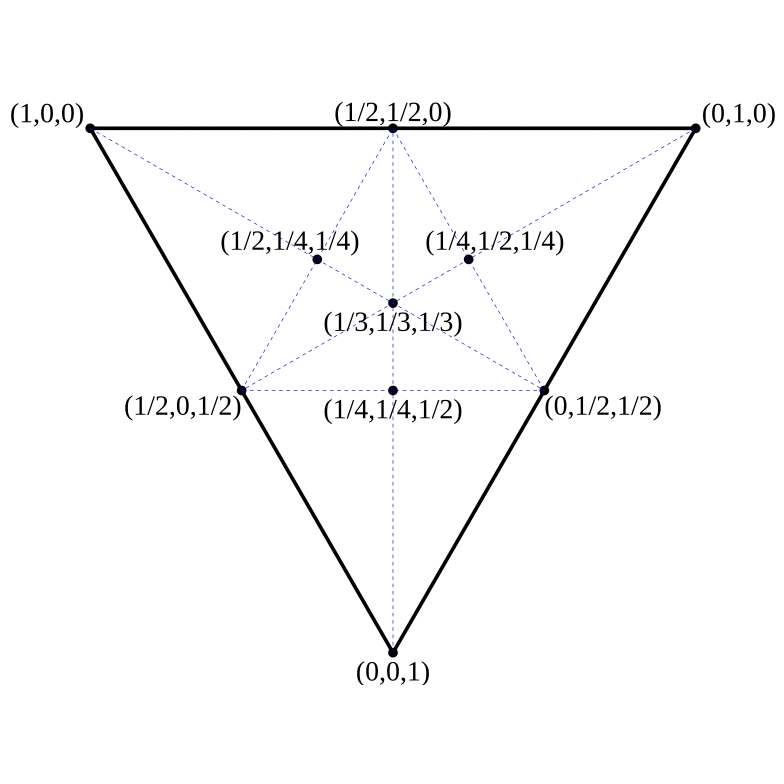
\includegraphics[width=.95\textwidth]{./immagini/bary1.png}
        \caption{}
        \label{fig:bary_a}
    \end{subfigure}
    \hfill
    \begin{subfigure}[b]{0.33\textwidth}
        % bary2
        \includegraphics[width=.95\textwidth]{./immagini/bary2.png}
        \caption{}
        \label{fig:bary_b}
    \end{subfigure}
    \caption{a) Geometrical construction, b) smooth interpolation of baricentric coordinates}
    \label{fig:bary}
\end{figure}

Notice that this process is applied to each triangle that composes the model, meaning that it can become a heavy computation very quickly. This is the case where the parallelised computation of powerful graphics processing units (GPUs) proves useful.

\paragraph{Depth test and overalapping: }

Once we have more than one triangle there might be overlapping, and to address this issue, we use a ray-tracer simulating technique to test how far a triangle is respect to the camera. In this way we can correctly identify which triangle should actually be part of the simulated nanostructure, see Fig. \ref{fig:depth}.

This process will be speed up incredibly by using the standard graphical pipeline used in the video-games industry, backed up by the physical and mathematical correctness of the ray-tracer approach.

Using this method, we can correctly simulate the nanoparticles discussed in the following chapters.

\begin{figure}[ht]
    \centering
    \begin{subfigure}[b]{0.32\textwidth}
        % depth
        \includegraphics[width=.95\textwidth]{./immagini/depth.png}
        \caption{}
        \label{fig:depth_a}
    \end{subfigure}
    \hfill
    \begin{subfigure}[b]{0.32\textwidth}
        % depth2
        \includegraphics[width=.95\textwidth]{./immagini/depth2.png}
        \caption{}
        \label{fig:depth_b}
    \end{subfigure}
    \hfill
    \begin{subfigure}[b]{0.32\textwidth}
        % depth3
        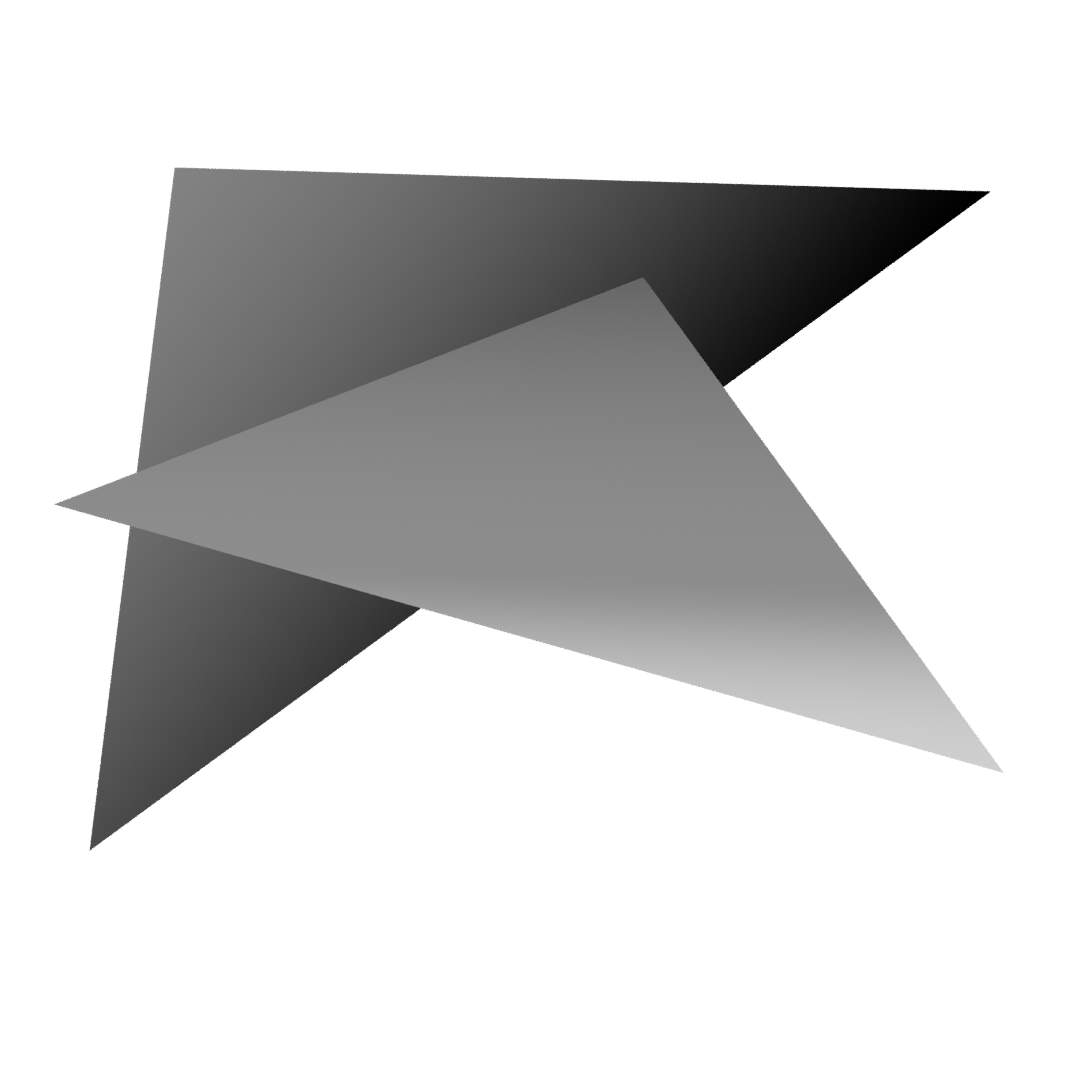
\includegraphics[width=.95\textwidth]{./immagini/depth3.png}
        \caption{}
        \label{fig:depth_c}
    \end{subfigure}
    \caption{a) A pair of triangles of unknown Z height b) Zoom of the overlapping surface c) Final result, obtained from comparing the depth at which each pixel is located}
    \label{fig:depth}
\end{figure}